\documentclass[../report.tex]{subfiles}

\begin{document}

% Chapter State of the art
% - Concepts (before diving into the protocoles, it is important to understand some concepts)
% - Outlines of the KAPE landscape (all PAKEs, history, overview)
% - Mains PAKEs (differences, improvement, tableau comparatif, pas besoin de décrire les constructions)
%   - EKE
%   - SRP
%   - OPAQUE
%   - KHAPE
% - PAKE choice (and reasons)

% (Attack on PAKEs ?)


% Chapter OPAQUE or Chapter KHAPE (depending on the PAKE choice)
% - detail construction (protocol) of the choosen PAKE

\chapter{State of the art}

\section{History of PAKEs}
\paragraph{EKE and variants (PAK, PPK, PAK-X)}
\paragraph{OKE}
\paragraph{SNAPI}
\paragraph{PEKEP}
\subsection{Symmetric PAKE}
\subsection{Asymmetric PAKE}
\paragraph{SRP}
\subsection{Strong asymmetric PAKE}
\paragraph{OPAQUE (2018)}
\paragraph{KHAPE (2021)}





\section{Main PAKEs}

\subsection{\writingFormulationBrut{OPAQUE}}


\paragraph{\writingFormulationBrut{Design}}
Jarecki and al. \cite{}. introduce the definition of Strong aPake (SaPAKE): an aPake secure against pre-computation attacks.

They provides two modular constructions, called the OPAQUE protocol that allow to builds SaPake protocols. The first construction allow to enhance any aPake to a SaPAKE while the second allow to enhance any Authenticated Key-Exchange (AKE) protocol (that are secure against KCI attacks) to an SaPAKE.
The security of these two construction is based on Oblivious PRF (OPRF) functions \cite{}.

These functions allow for each party, namely the client and the server, to input a secret value and then the client can use the output as a key. Neither party can learn the other party's secret and the server cannot learn the output of the function.

Overall, the OPAQUE protocol allow to secure authentication from the simplest applications to the most sensitive ones.


\begin{figure}[h]
 \centering
 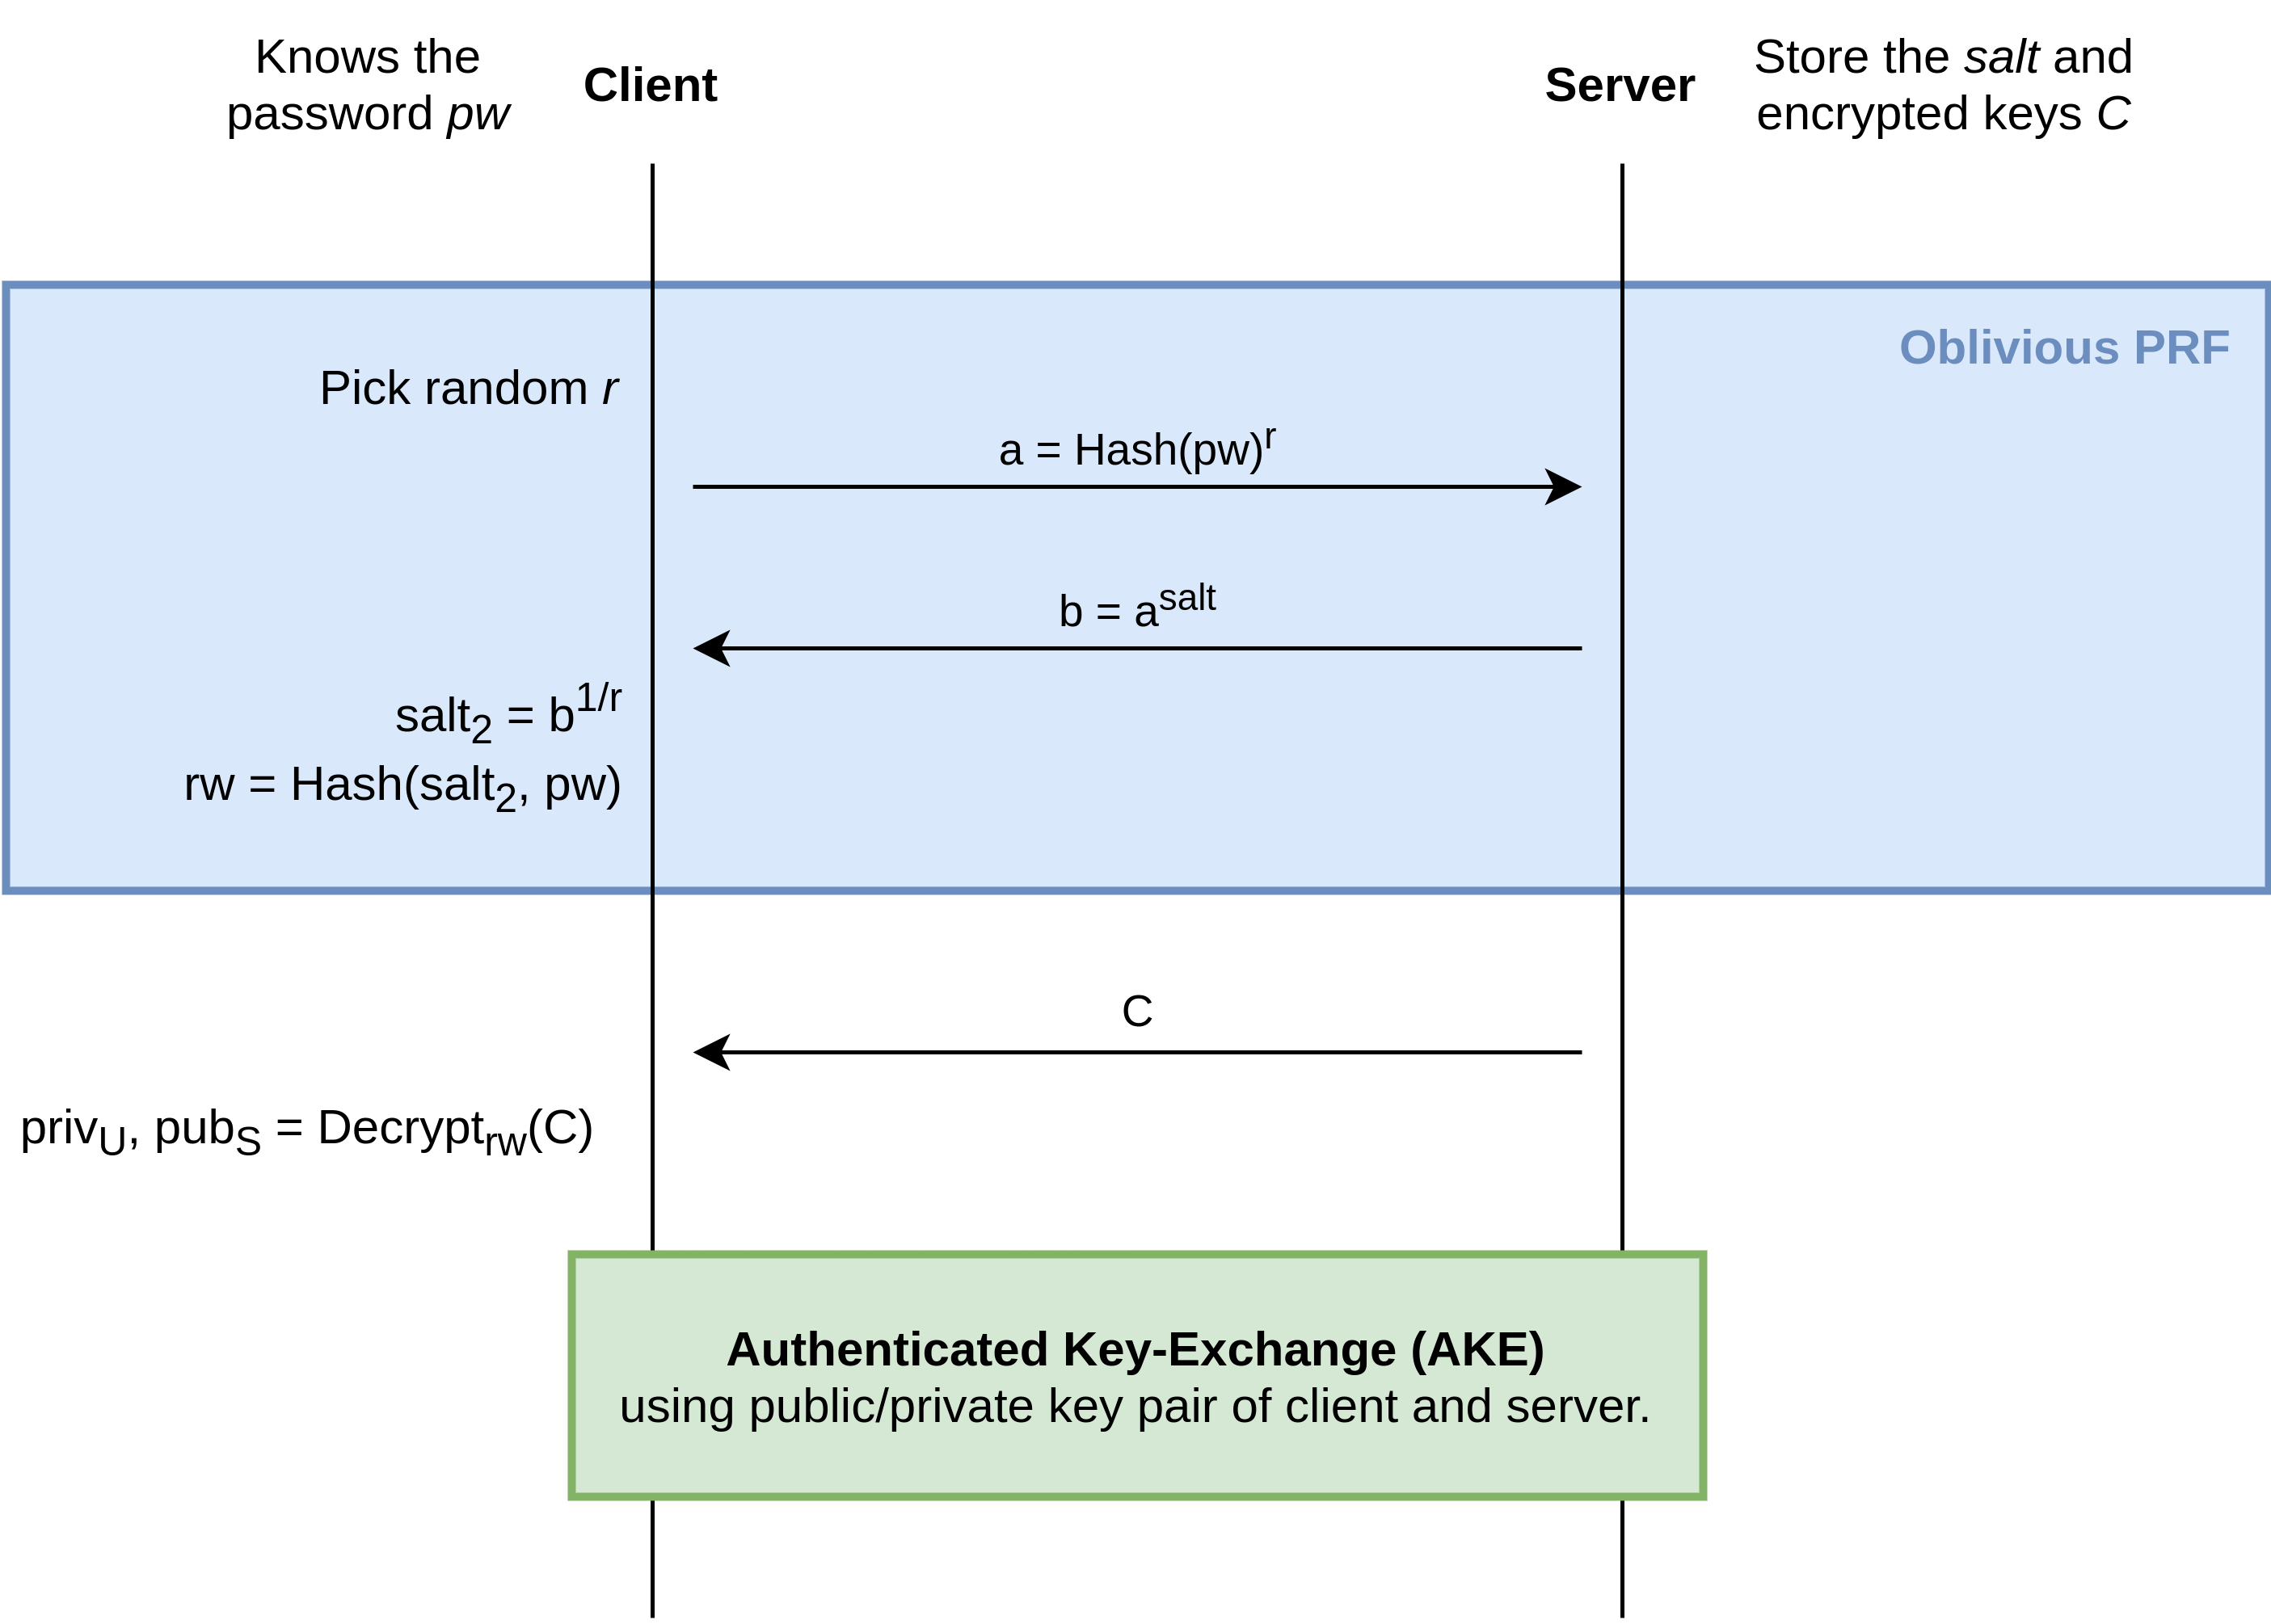
\includegraphics[width=\textwidth]{OPAQUE.png}
 % OPAQUE.png: 2166x1206 px, 72dpi, 76.41x42.54 cm, bb=0 0 2166 1206
 \caption{Login process with OPAQUE protocol using OPRF and AKE.}
 \label{fig:OPAQUE_AKE}
\end{figure}




\paragraph{\writingFormulationBrut{Construction}}

Figure \ref{fig:OPAQUE_AKE} shows the OPAQUE protocol using OPRF and AKE during login process.
The steps are the following :

(1) Generate a random value r to blind the hash of password so that the server cannot retrieve the password from the mapping.
(2) Send result to server
(3) Server add the salt to the password
(4) Client calculate the exponant of the inverse of r to unblind the value. He canno't retrieve salt.
(5) With the secret salt salt2, client compute secret key sk.
(6) Server send encrypted keys ek to clients. ek contains server's public key and client's private key encrypted with sk.
(7) If the password entered is correct, client can use sk to decrypt ek and retrieve his private key privU
(8) With both keys, clients and server can run an authenticated key exchange for mutual authentication.

\paragraph{\writingNotes{Additional features}}

     "Supports user-side password hardening"
     "has a built-in facility for password-based storage-and-retrieval of secrets and credentials"
     "accommodates a user-transparent server-side threshold implementation"
     "far more secure alternative to the practice of deriving low-entropy secrets directly from a user's password"


\paragraph{\writingFormulationBrut{Register}}
When a client want to register, the client generate a public/private key pair. He then encrypt his private key and the server's public key with the secret key (OPRF's output).
$C = Encrypt_rw_(client's private key | server's public key)$

Then he send the ciphertext to the server to store.


\paragraph{\writingFormulationBrut{Login}}
For the login phase, the client enter it's password in the OPRF and the server send the ciphertext to the client.
If the password entered is correct, the client can decrypt the ciphertext with OPRF output to obtain his private key and the server's public key.
He then use these keys to run a authenticated key exchange with the server (like HMQV ?).

In the other hand, if the password is wrong, the OPRF output is totally different and the ciphertext decryption make the keys uncorrect and the server will refuse it during the key exchange (?). % TODO confirmation




\section{\writingNotes{Comparing mains solutions}}

This section compare the mains PAKEs on their security guarantees and performances. Details and comments on each criteria can be found on Section \ref{sec:comparison_details}.

\begin{center}
   \begin{tabular}{ | c | p{8cm} || p{1cm} | p{1cm} | p{2cm} | p{2cm} | }
     \hline
     \textbf{\#} & \textbf{Criteria} & \textbf{EKE} & \textbf{SRP} & \textbf{OPAQUE} & \textbf{KHAPE} \\ \hline
     
     % Content :
     
     % Qualities (security guarantees)
     
     10 & Server doesn't store password in cleartext & x & x & Yes & x \\ \hline
     1 & Avoid sending cleartext password to the server & x & x & Yes & x \\ \hline
     2 & Secure against pre-computation attacks & x & x & Yes & x \\ \hline
     3 & Server doesn't send salt in cleartext & x & x & Yes & x \\ \hline
     4 & Forward secrecy & x & x & Yes & x \\ \hline
     5 & Mutual authentication & x & x & Yes & x \\ \hline
     6 & PKI-free & x & x & Yes, except during register & x \\ \hline
     7 & User-side password hardening & x & x & Yes & x \\ \hline
     8 & Built-in mechanism to store client's secrets on the server & x & x & Yes & x \\ \hline
     9 & Server threshold implementation & x & x & Yes, user-transparent & x \\ \hline
     11 & Resistant upon Oblivious PRF compromise & x & x & No, entire security is compromised & Fall back to non-strong aPAKE \\ \hline
     12 & Internet standard & x & x & Draft & x \\ \hline
     13 & Security proof & x & x & Yes, in a very strong model & x \\ \hline
     
     % Performances
     
     14 & Easily adaptable to elliptic curves & x & x & Yes & x \\ \hline
     15 & Number of messages & x & x & 3 ? & x \\ \hline
     16 & Number of exponentiations & x & x & 3 or 4 ? & x \\ \hline
     17 & Patented & x & x & x & x \\ \hline
     18 & Release date & x & x & x & x \\ \hline
     19 & Version & x & x & x & x \\ \hline
     20 & Got broken & x & x & x & x \\ \hline

     \end{tabular}
 \end{center}
 
\subsection{Details} \label{sec:comparison_details}



\paragraph{\writingFormulationClean{10. Server doesn't store password in cleartext.}}
This is the main security property of asymmetric PAKE \cite{aPAKE_Formalized}. Server doesn't have to store password in cleartext which should make it more resilient in case of server compromise. Adversary has to compute an offline attack to retrieve passwords from the compromised server.

\paragraph{\writingFormulationBrut{1. Avoid sending password in cleartext to the server.}}
Even though it seems similar to criteria 1, it's not. Criteria 1 is about password storage but this criteria is about password transmission. Transmissions and storage of the password are vulnerable to different attacks vectors.
The server don't receive password in cleartext which avoid any miss-handling vulnerabilities such as logging or caching cleartext password on the server.

\paragraph{\writingFormulationClean{2. Secure against pre-computation attacks.}}
This is the main security property of Strong aPAKE \cite{OPAQUE_Paper}. The server doesn't leak any data (generally the salt) that could allow an attacker to perform a pre-computation attack. This attack allow an attacker to compute a table \emph{before} the server even get compromised. Once the attacker succeed in compromising the server, he can use the pre-computed table to retrieve the passwords \emph{instantaneously}. So this protection force the attacker to perform an offline dictionary attack after successful server compromise. % This vulnerability weaken the initial benefit of using an aPAKE \cite{aPAKE_Formalized} and even make password-over-TLS more secure \cite{OPAQUE_Paper} (than aPAKE vulnerable to pre-computation attacks).

\paragraph{\writingNotes{3. Server doesn't send salt in cleartext.}}
Same as 2.

\paragraph{\writingFormulationClean{4. Forward secrecy.}}
In key-exchange protocol, Forward Secrecy (also called Full Forward Secrecy or Perfect Forward Secrecy) ensure that upon compromise of any long term key used to negotiate sessions key, an attacker cannot compromise previous session keys.
In details key-exchange protocol use long-lived keys to authenticate the user and short-lived keys to encrypt sessions. With Forward Secrecy, an attacker that successfully compromised a long-lived key cannot retrieve any previous session data even if he recorded the previous encrypted transmissions. % TODO cite Duc CAA 05-password ?

\paragraph{\writingFormulationClean{5. Mutual authentication.}}
Mutual authentication explicit that user must be authenticated to the server but also that the server must authenticate itself to the user to avoid that an adversary impersonate the server to maliciously communicate with the client.

\paragraph{\writingFormulationBrut{6. PKI-free.}}
The transmissions between client and server doesn't require to be secured with PKI. This is a big improvement over classical authentication method (Password-over-TLS) considering the occurrence of PKI failures nowadays. % "PKI failures include stealing of server private keys, software that does not verify certificates correctly, users that accept invalid or suspicious certificates, certificates issued by rogue CAs, servers that share their TLS keys with others e.g., CDN providers or security monitoring software, information (including passwords) that traverses networks in plaintext form after TLS termination; and more."

\paragraph{\writingFormulationClean{7. User-side password hardening.}}
User can use password hardening technique to increase the cost of an offline attacks if the server get compromised. This is done by using ressource-heavy functions such as Scrypt \cite{Scrypt_Paper} or Argon2 \cite{Argon2_Paper} instead of computing a simple and efficient hash. These functions allows to drastically slows down hashing process and so making offline attacks and online guessing attack much slower.

\paragraph{\writingNotes{8. Built-in mechanism to store client's secrets on the server.}}
OPAQUE "has a built-in facility for password-based storage-and-retrieval of secrets and credentials"

\paragraph{\writingNotes{9. Server threshold implementation.}}
OPAQUE "accommodates a user-transparent server-side threshold implementation"

\paragraph{\writingNotes{11. Resistant upon Oblivious PRF compromise.}}
``There is a significant difference in the reliance on the security of
OPRF. While the password security of OPAQUE breaks down with a
compromise of the OPRF key (namely, it allows for an offline dictionary attack
on the password), in KHAPE the effect of compromising the OPRF is only to
fall back to the (non-strong) aPAKE setting. In particular, this distinction is
relevant in the context of quantum-safe cryptography as there are currently no
known efficient OPRFs considered to be quantum safe. This opens a path to
quantum-safe aPAKEs based on KHAPE with key hiding quantum-safe KEMs.'' \cite{OPAQUE_Paper}.

\paragraph{12. Internet standard.}

\paragraph{\writingNotes{13. Security proof.}}
OPAQUE "security proof in a very strong model"

\paragraph{14. Easily adaptable to elliptic curves.}


\paragraph{15. Number of messages.}


\paragraph{16. Number of exponentiations.}


\paragraph{17. Patented.}


\paragraph{18. Release date.}


\paragraph{19. Version.}


\paragraph{20. Got broken.}



\end{document}
